\documentclass[a4paper,11pt]{article}
\usepackage{a4wide,graphicx,amssymb, amstext, amsmath, epstopdf, booktabs, verbatim, geometry, appendix, natbib, lmodern, tabularx, enumitem, longtable, hyperref, subcaption, usecases}

%\geometry{letterpaper}
%\usepackage{garamond}

\newcommand*\Title{Trafic Control System}
\newcommand*\cpiType{User Requirements Document}
\newcommand*\Author{}
\title{\Title}
\author{}
\date{\today}
%-----------------------------------------------------------

\usepackage{template/template} % This is what makes your document look like a cpi document.


\begin{document}

\begin{titlepage}
\maketitle
\end{titlepage}

  	\linespread{1.15} %Set standard document linespacing
    
  	\subsection*{Background and Context}
  	This user requirements document specifies the software requirements for the "Traffic Control System". This application allows traffic to be simulated with the purpose of noticing traffic jams related to traffic lights.
  	
  	\subsection*{Definitions and abreviations}
  	\begin{longtable}[l]{p{80pt} p{350pt}} 
  		User & The person who is controlling this application.\\
  		System & The implementation of this application.\\
  		Grid & A place on the screen where a component can be added for the traffic situation.\\
  		Component & A visible representation of an object on the screen of the user.\\
  		Crossing & A component that can be used in the traffic simulation which has traffic lights.\\
  		Traffic light & A component of the crossing which controlls the traffic by displaying colors red, yellow green. For which green the traffic is allowed to go.\\
  		Pedestrian & A simulation of a pedestrian crossing a road from the traffic light.\\
  		Lane & A component that represent a piece of road.\\
  		Group of lanes & A group of incoming lanes at a crossing which have green light at the same time.\\
  		Cars & A component that represent a car on the road.\\
  	\end{longtable}
  	
  	\tableofcontents
  	\newpage
  	
  	
  	\section{Requirements}
\subsection{General requirements}
\begin{tabularx}{\textwidth}{|p{2cm}X|}\hline
	Code & Requirement \\\hline
	GEN-010 & The program is compatible with Windows 7.\\\hline
	GEN-020 & The system allows to design a traffic situation.\\\hline
	GEN-020A & The traffic situation can be designed with the following components
	\begin{itemize}[noitemsep,nolistsep]
		\item Crossroad without pedestrian lane
		\item Crossroad with pedestrian lane
		\item Straight road
		\item Curved road
	\end{itemize}\\\hline
	GEN-020 & The amount of traffic comming from each lane can be changed.\\\hline
	GEN-030 & From the traffic lights of the crossroads it is possible to change the amount of time that traffic light is geen.\\\hline
	GEN-040 & The system allows simulate traffic, and allow to change the simulation speed.\\\hline
	GEN-050 & The sytem allows to open and save the traffic situation to a file.\\\hline
	GEN-050A & The sytem doesn't allow to save a simulation, it only saves the traffic situation.\\\hline
\end{tabularx}

\subsection{System requirements}


  	\section{Specification}
The following chapter describes the implementation of the application.
\subsection{Main window}
The main window is divided into two parts, see figure \ref{fig:mainwindow}. On the very top of the application is a menubar where the user can do actions like saving their work. Then the window is split up in two parts. On the left side is the menubar and on the right side the grid. The grid is the representation of the traffic situation. The components (see section \ref{sec:components}) can be dragged from the sidebar to the grid. To remove a component right-click on it and press on Delete in the context-menu. All open incoming lanes have a text-box which allows the user to specify the amount of traffic coming. The simulation can simply be started by the play button and the simulation speed can simply be changed with a slider. With the button "Show Report" the user can get a report of that moment of the simulation. The report will contain a still image of the current situation. It highlights the traffic jams and the image can be saved.

\begin{figure}[!ht]
	\caption{Mockup of the Main window}
	\label{fig:mainwindow}
	\centering
	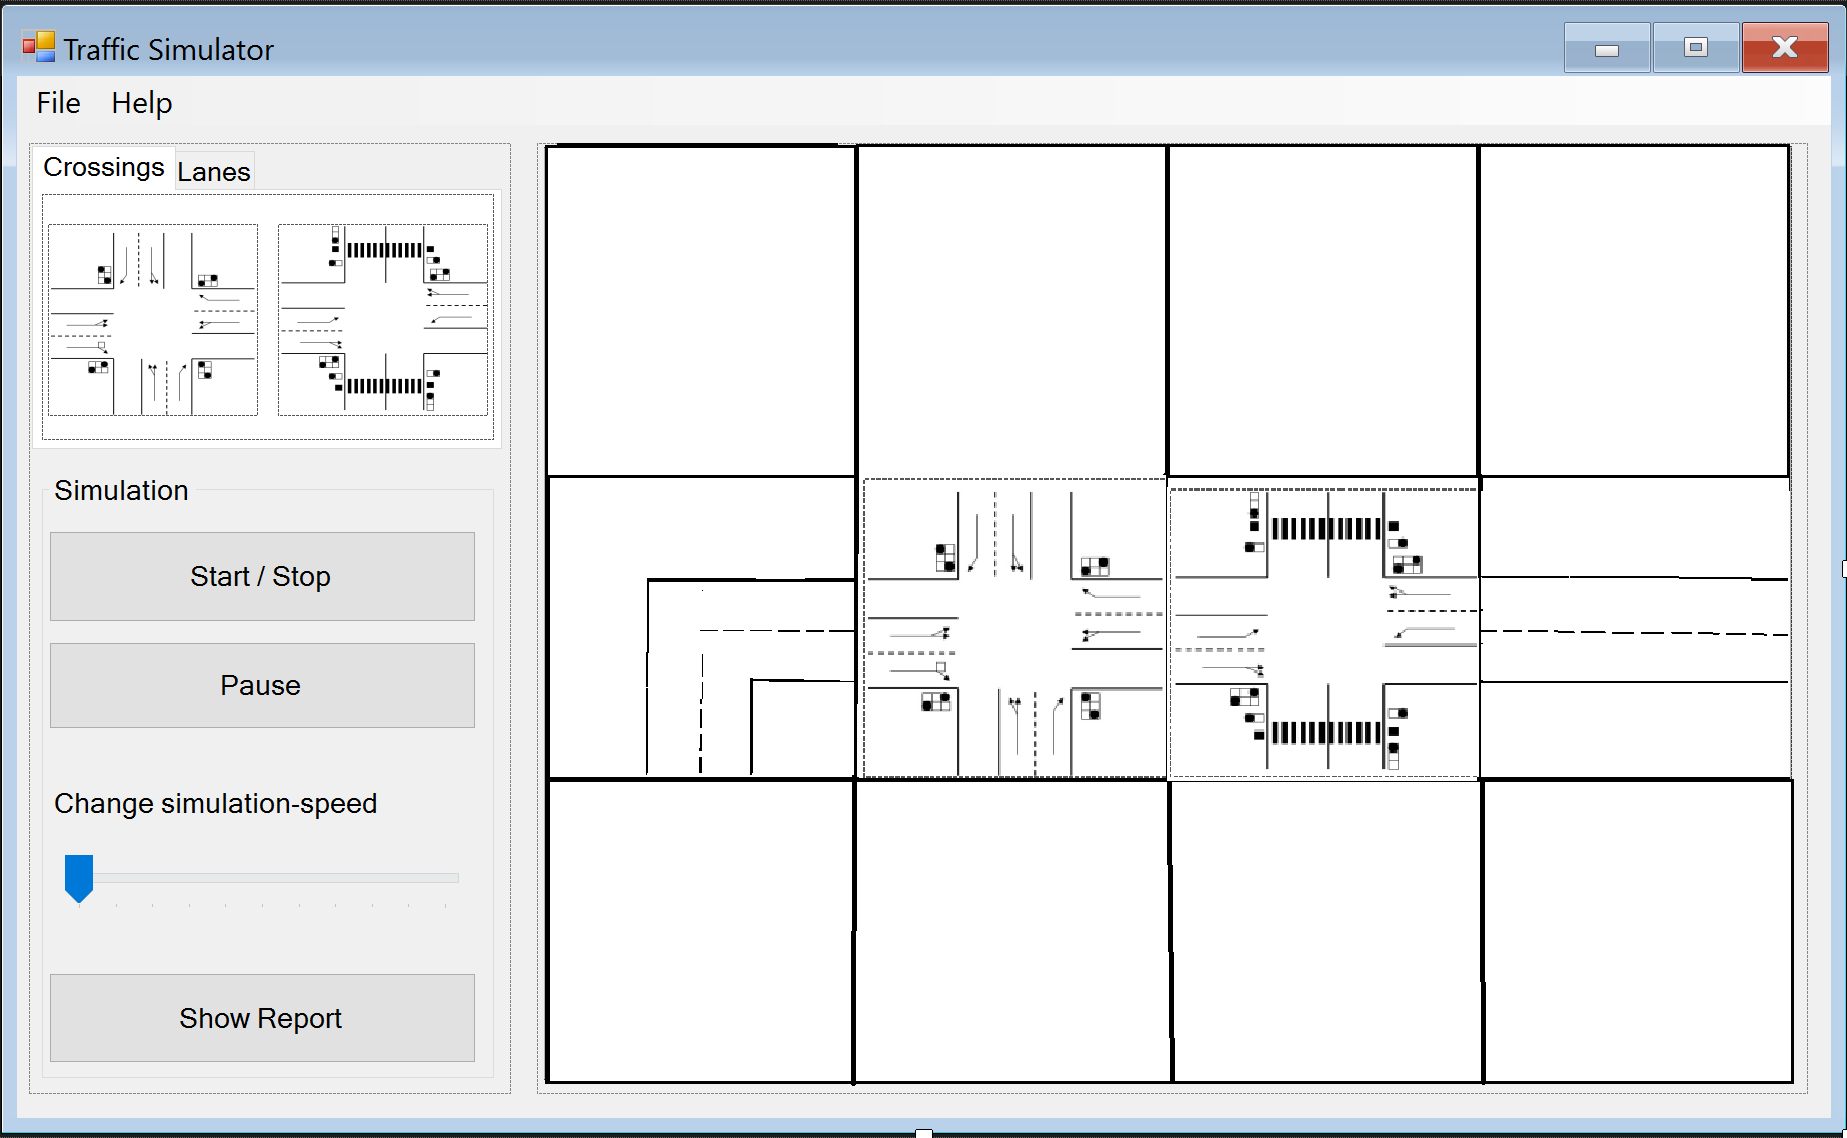
\includegraphics[width=0.8\textwidth]{figures/MainForm}
\end{figure}
\begin{figure}[!ht]
	\caption{Mockup of the Configuration window}
	\label{fig:Configurationwindow}
	\centering
	\includegraphics[width=0.8\textwidth]{figures/configurationForm}
\end{figure}
\begin{tabularx}{\textwidth}{|p{0.5cm}p{2cm}X|}\hline
	Rxx & Code & Specification \\\hline
	R01 & MWS-010 & When the application just started it will create a new grid 4x3\\\hline
	R01 & MWS-020 & The main window has a menubar.\\\hline
	R01 & MWS-020A & The menu bar has the following structure:
	\begin{itemize}[noitemsep,nolistsep]
		\item File
		\begin{itemize}
			\item New
			\item Open
			\item Save
			\item Save As
		\end{itemize}
		\item Help
	\end{itemize}\\\hline
	R01 & MWS-020B & A new simulation can be started by pressing on new, a window will prompt for the width and height for the size of the grid.\\\hline
	R01 & MWS-020C & The manual can be opened by pressing on Help.\\\hline
	R01 & MWS-030 & The window has a sidebar on the left.\\\hline
	R01 & MWS-032 & The sidebar contains all the components described in section \ref*{sec:components}.\\\hline
	R01 & MWS-032A & The component can be added to the grid by dragging it to the desired location.\\\hline
	R01 & MWS-034 & The sidebar contains a button which allows the simulation to start/stop.\\\hline
	R01 & MWS-035 & The sidebar contains a button which allows the simulation to pause.\\\hline
	R01 & MWS-036 & The simulation-speed can be changed by adjusting the slider.\\\hline
	R02 & MWS-038 & In simulation the button "Show report" will generate a report.\\\hline
	R01 & MWS-038A & The report is shown in a new window and contains the current traffic situation including cars and pedestrians.\\\hline
	R01 & MWS-038B & In the report the traffic jams are highlighted.\\\hline
	R01 & MWS-038C & The report can be saved as an image file.\\\hline
\end{tabularx}

To change the amount of time each traffic light is green press right-click on the crossroad and click in the context-menu on "Traffic-light configuration". A new window will pop up which allows to set the time for each group of lanes.

\begin{tabularx}{\textwidth}{|p{0.5cm}p{2cm}X|}\hline
	Rxx & Code & Specification \\\hline
	R01 & MWS-100 & All open incoming lanes have a textbox to specify the amount of traffic coming in.\\\hline
	R01 & MWS-110 & When pressing right-click on any component placed on the grid a context-menu appears which allows to rotate or delete the component.\\\hline
	R01 & MWS-120 & When pressing right-click on a crossroad it gives an option "Traffic-light configuration"\\\hline
	R01 & MWS-120A & A new window will pop-up with a list of all the lane groups.\\\hline
	R01 & MWS-120B & The user can select a lane group and change the amount of time the traffic-light is green.\\\hline
\end{tabularx}

\newpage
\subsection{Components}
\label{sec:components}
\subsubsection{Crossroad}
\begin{figure}
	\centering
	\begin{subfigure}{.5\textwidth}
		\centering
		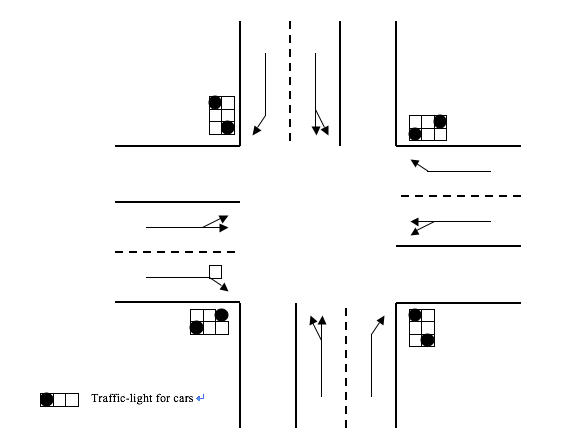
\includegraphics[width=\linewidth]{figures/crosswaya.png}
		\caption{Crossroad without pedestrians.}
		\label{fig:crossa}
	\end{subfigure}%
	\begin{subfigure}{.5\textwidth}
		\centering
		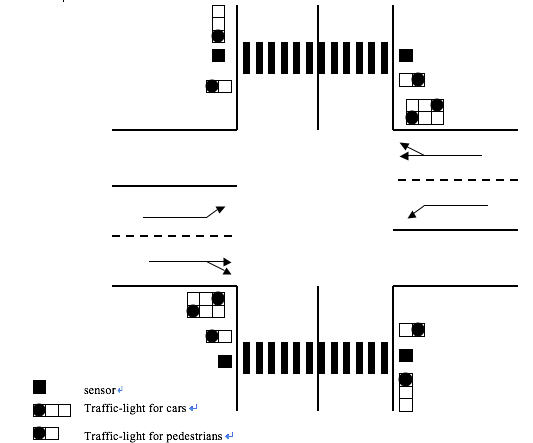
\includegraphics[width=\linewidth]{figures/crosswayb.png}
		\caption{Crossroad with pedestrians.}
		\label{fig:crossb}
	\end{subfigure}
	\caption{Crossways}
	\label{fig:cross}
\end{figure}

\begin{tabularx}{\textwidth}{|p{0.5cm}p{2cm}X|}\hline
	Rxx & Code & Specification \\\hline
	R01 & CWC-010 & All cossways are connected to 4 roads\\\hline
	R01 & CWC-020 & There are 2 different types of crossroads see figure \ref{fig:cross}.\\\hline
	R01 & CWC-020 & Type A crossroad is without pedestrian lane.\\\hline
	R01 & CWC-020A & From each side the crossroad A has 2 incoming lanes and 1 outgoing lane.\\\hline
	R01 & CWC-025 & Type B crossroad is with an pedestrian lane.\\\hline
	R01 & CWC-025A & Type B has from 2 opposite sides a crossroad for pedestrians, which only has 1 incoming lane.\\\hline
	R01 & CWC-030 & Traffic light for cars have the colors red, orange and geen.\\\hline
	R01 & CWC-035 & Traffic light for pedestrians have the colors red and green.\\\hline
	R01 & CWC-040 & Traffic light for cars only turn orange after green.\\\hline
	R01 & CWC-040A & Amount of time for the orange light is fixed, and is set to 2 seconds in normal simulation time.\\\hline
	R01 & CWC-045 & Traffic light for green are set to default for 4 seconds.\\\hline
	R01 & CWC-045A & The amount of time each light group of an crossroad can be changed.\\\hline
	R01 & CWC-050 & The order of the light groups are fixed.\\\hline
	R01 & CWC-050A & When there are no cars or pedestrians on the sensors for the according lightgroup it will be skipped in the simulation.\\\hline
	R01 & CWC-060 & Unconnected incoming lanes have a textbox which allows to change the number of cars comming in when the simulation is running.\\\hline
\end{tabularx}

\newpage
\subsubsection{Road}
\begin{figure}
	\centering
	\begin{subfigure}{.5\textwidth}
		\centering
		\includegraphics{figures/laneaa.png}
		\caption{Straight road.}
		\label{fig:strr}
	\end{subfigure}%
	\begin{subfigure}{.5\textwidth}
		\centering
		\includegraphics{figures/lanebb.png}
		\caption{Curved road.}
		\label{fig:curvedr}
	\end{subfigure}
	\caption{Crossways}
	\label{fig:road}
\end{figure}

\begin{tabularx}{\textwidth}{|p{0.5cm}p{2cm}X|}\hline
	Rxx & Code & Specification \\\hline
	R01 & RCP-010 & There are two types of roads, a straight road and a curved road.\\\hline
	R01 & RCP-020 & All roads have 2 lanes, in both directions.\\\hline
	R01 & RCP-030 & Unconnected incoming lanes have a textbox which allows to change the number of cars comming in when the simulation is running.\\\hline
	R01 & RCP-030A & Just like crossroad see CWC-060.\\\hline
\end{tabularx}

\subsubsection{Car}
\begin{tabularx}{\textwidth}{|p{0.5cm}p{2cm}X|}\hline
	Rxx & Code & Specification \\\hline
	R01 & CAR-010 & All cars run at the same speed, the speed allows 1 car to pass the green light per second.\\\hline
	R01 & CAR-020 & Cars do not collide.\\\hline
	R01 & CAR-020A & Cars hold distance from each other when driving.\\\hline
	R01 & CAR-030 & No cars go through red light.\\\hline
	R01 & CAR-040 & Cars will not go through orange light, in case the car is in front of the traffic light.\\\hline
	R01 & CAR-050 & Cars will take a random direction on the crossroad.\\\hline
	R02 & CAR-060 & Cars accerlate and break at a realistic speed.\\\hline
\end{tabularx}

\subsubsection{Pedestrian}
\begin{tabularx}{\textwidth}{|p{0.5cm}p{2cm}X|}\hline
	Rxx & Code & Specification \\\hline
	R01 & PED-010 & Pedestrians have 50\% change on being at the crosswalk.\\\hline
	R01 & PED-020 & Nothing can be configured of the pedestrians.\\\hline
\end{tabularx}

\newpage
\subsection{Traffic light groups}
\begin{figure}
	\centering
	\begin{subfigure}{.5\textwidth}
		\centering
		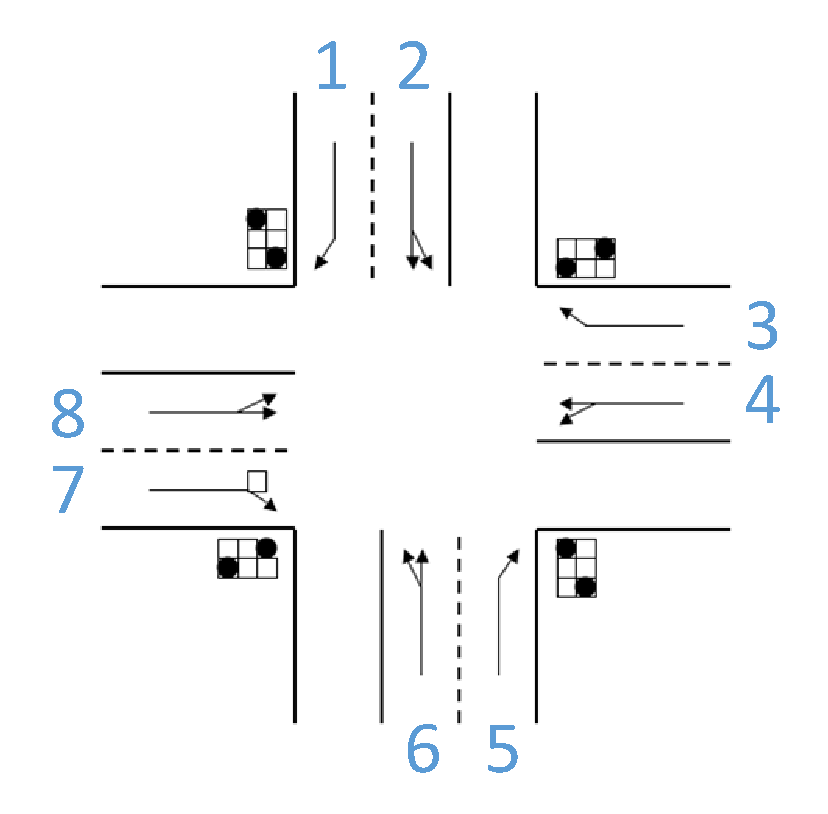
\includegraphics[width=0.8\textwidth]{figures/CrossroadAL.pdf}
		\caption{Crossroad A incoming lane numbers.}
		\label{fig:cral}
	\end{subfigure}%
	\begin{subfigure}{.5\textwidth}
		\centering
		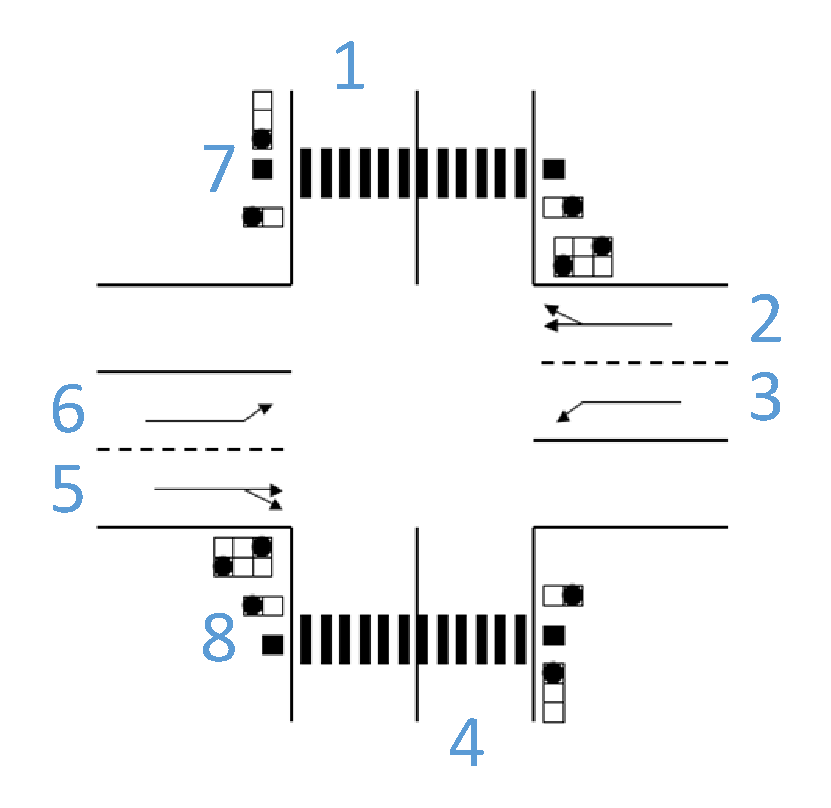
\includegraphics[width=0.8\textwidth]{figures/CrossroadBL.pdf}
		\caption{Crossroad B incoming lane numbers.}
		\label{fig:crbl}
	\end{subfigure}
	\caption{Crossways}
	\label{fig:tlg}
\end{figure}

The group of lanes which have green light at the same moment are defined in this section. The traffic lights follow the order as defined in this document, Traffic lights will skip a light group if no cars are present on the group of lanes.

\subsubsection{Crossroad A}
\begin{tabularx}{\textwidth}{|p{0.6cm}p{4cm}X|p{0.6cm}p{4cm}X|}\hline
	ID & Image & Lanes & ID & Image & Lanes \\\hline
	A1 &  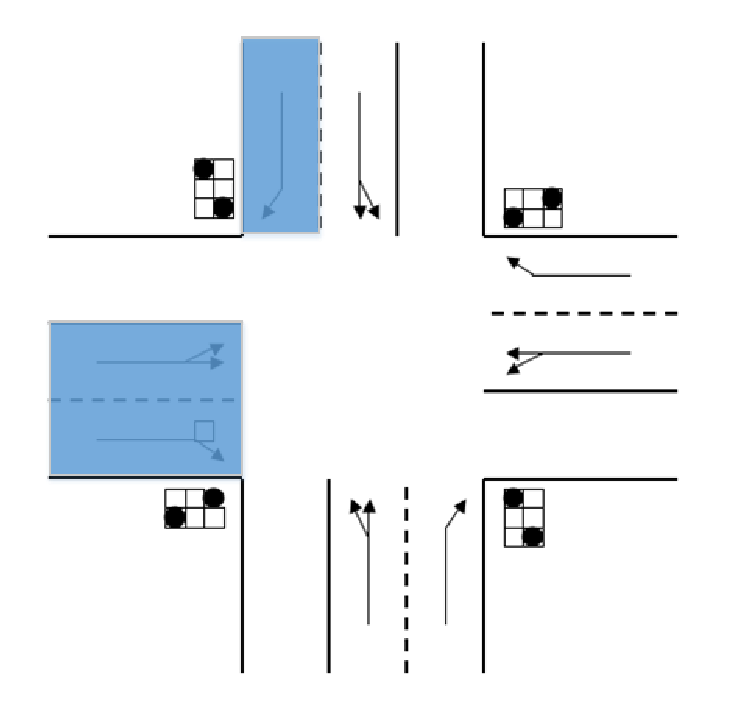
\includegraphics[width=4cm]{figures/CrossroadA1.pdf} & 1, 7, 8 &
	A2 &  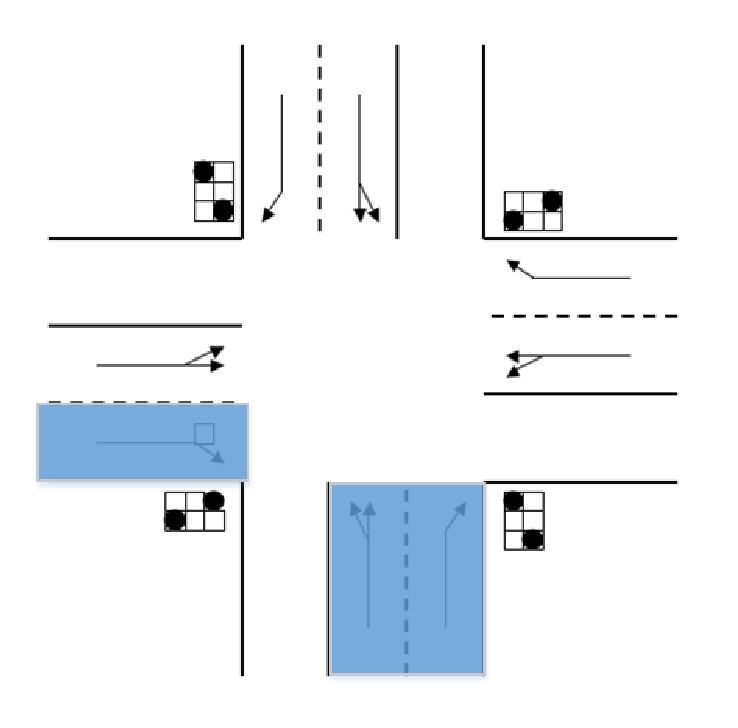
\includegraphics[width=4cm]{figures/CrossroadA2.pdf} & 5, 6, 7 \\\hline
	A3 &  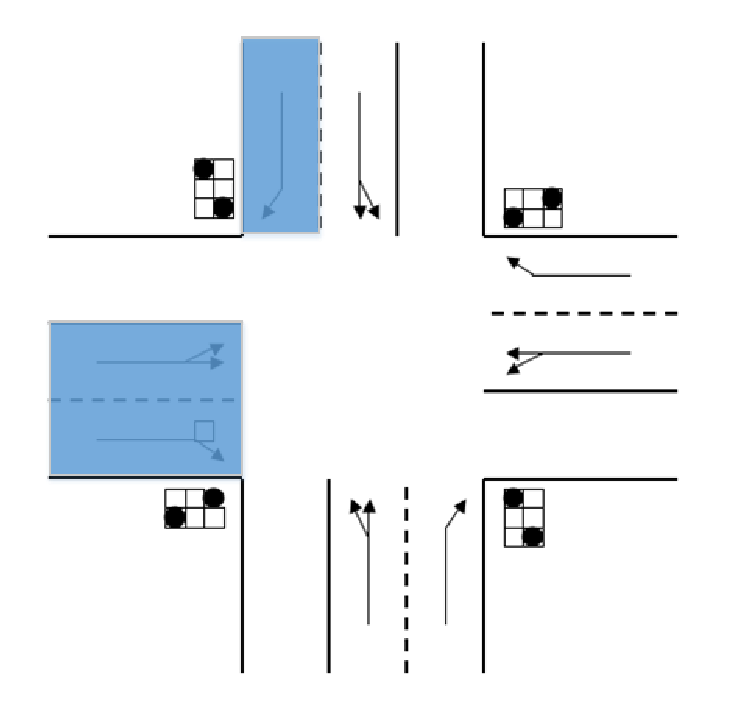
\includegraphics[width=4cm]{figures/CrossroadA3.pdf} & 3, 4, 5 &
	A4 &  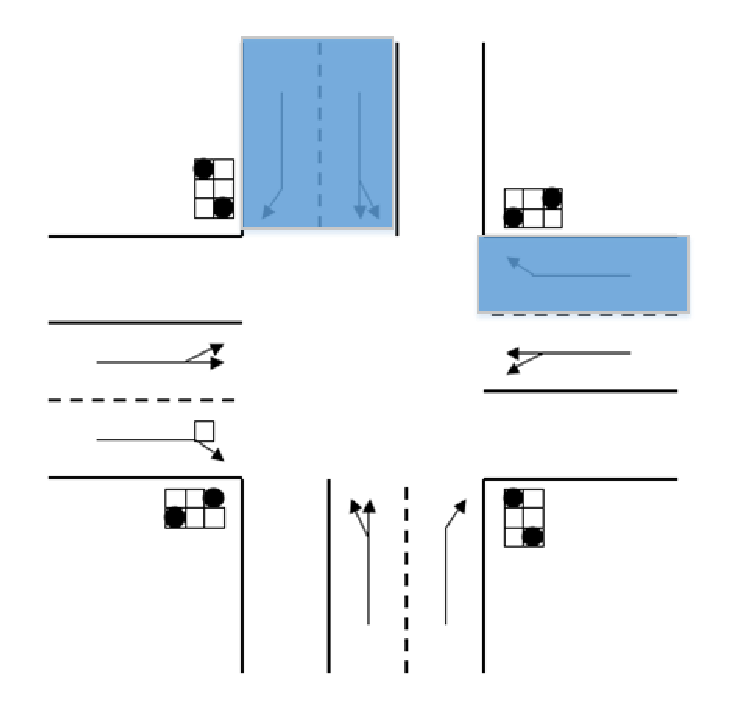
\includegraphics[width=4cm]{figures/CrossroadA4.pdf} & 1, 2, 3 \\\hline
\end{tabularx}

\subsubsection{Crossroad B}
\begin{tabularx}{\textwidth}{|p{0.6cm}p{4cm}X|p{0.6cm}p{4cm}X|}\hline
	ID & Image & Lanes & ID & Image & Lanes \\\hline
	A1 &  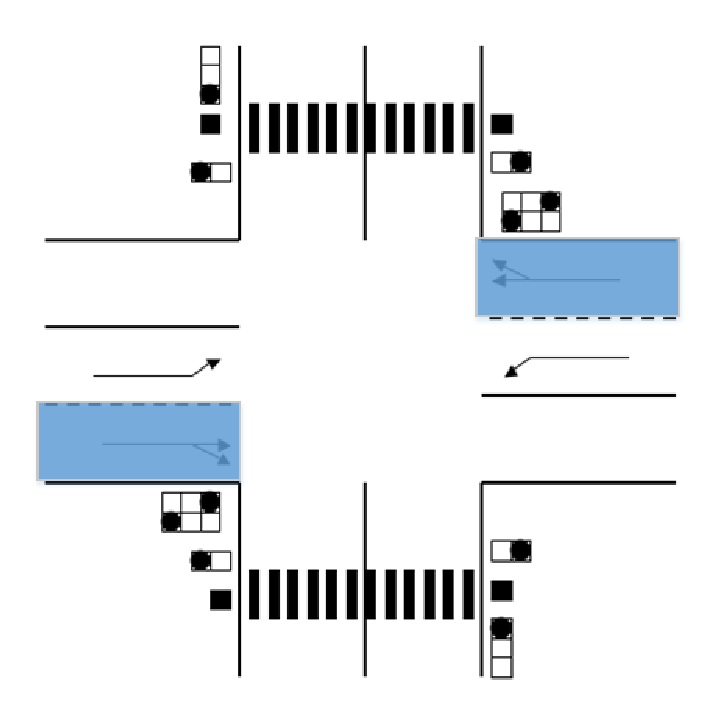
\includegraphics[width=4cm]{figures/CrossroadB1.pdf} & 2, 5 &
	A2 &  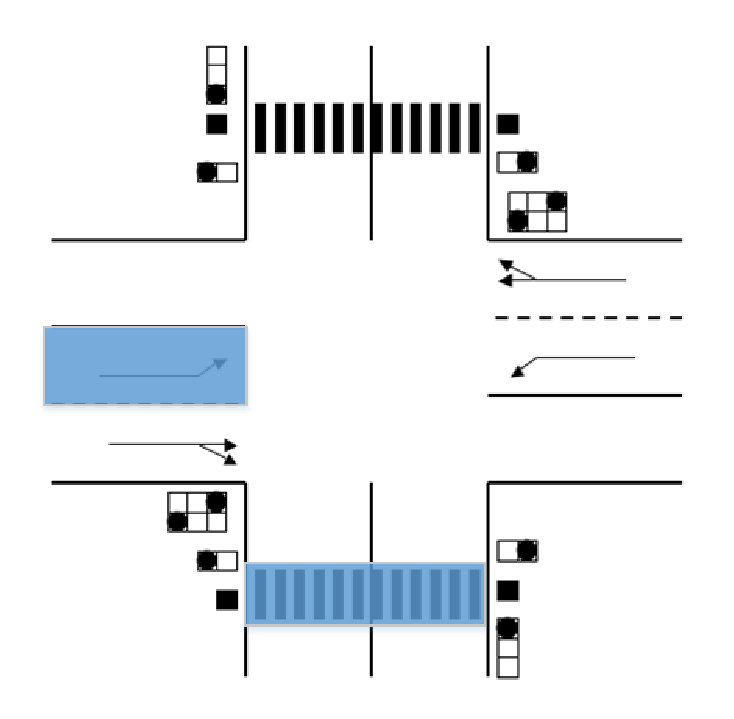
\includegraphics[width=4cm]{figures/CrossroadB2.pdf} & 6, 8 \\\hline
	A3 &  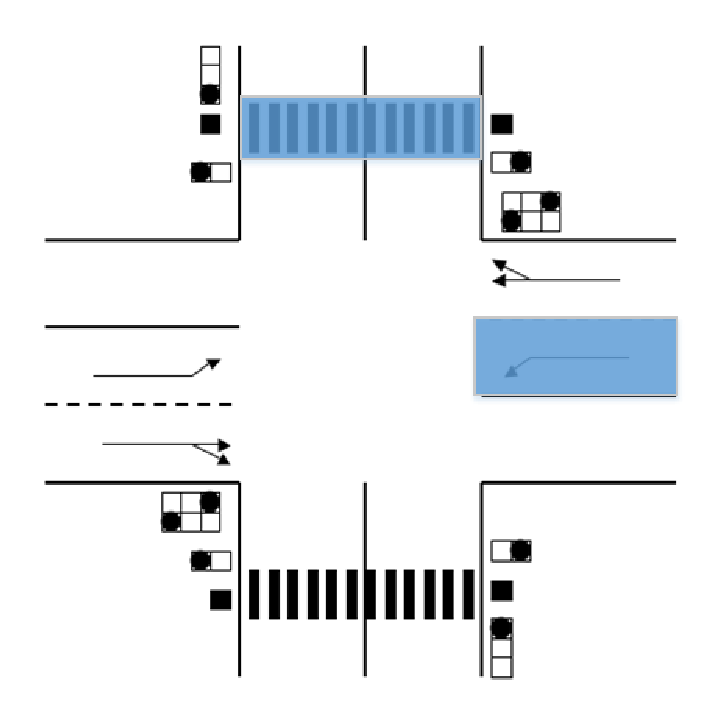
\includegraphics[width=4cm]{figures/CrossroadB3.pdf} & 3, 7 &
	A4 &  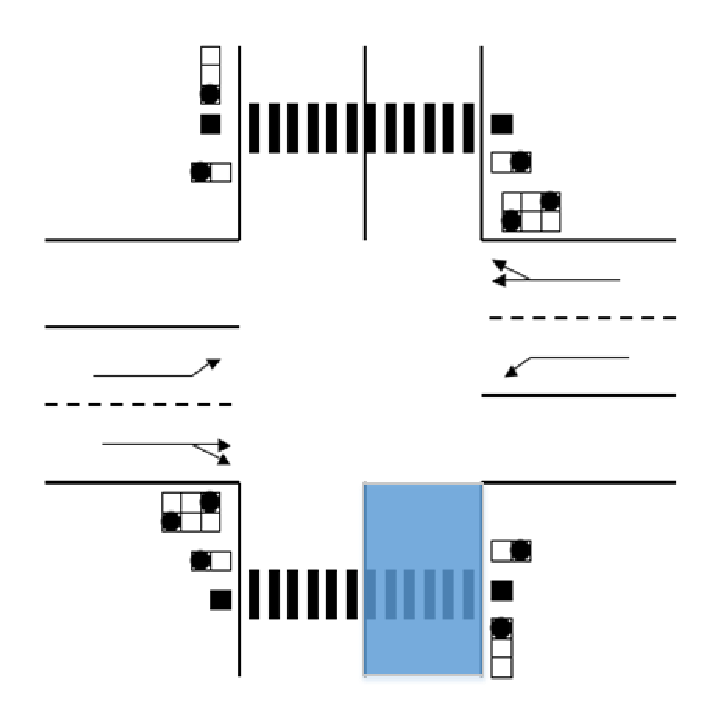
\includegraphics[width=4cm]{figures/CrossroadB4.pdf} & 4 \\\hline
	A4 &  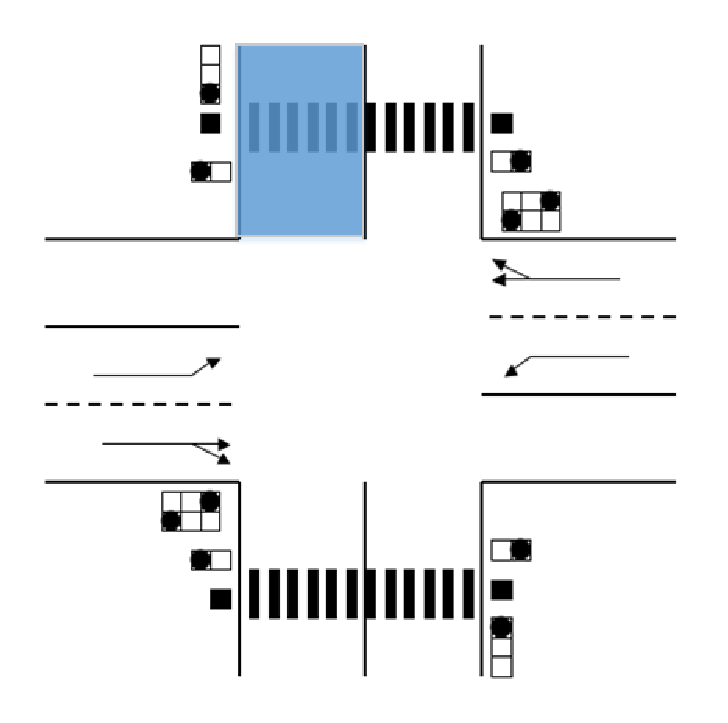
\includegraphics[width=4cm]{figures/CrossroadB5.pdf} & 1 & & & \\\hline
\end{tabularx}

    \section{Use cases}
\begin{usecase}
	
	\addtitle{Use Case 1}{Positioning a lane} 
	
	%Level: "user-goal" or "subfunction"
	\addfield{Level:}{User-goal}
	
	%Primary Actor: Calls on the system to deliver its services.
	\addfield{Primary Actor:}{End-User}
	
	%Preconditions: What must be true on start and worth telling the reader?
	\addfield{Preconditions:}{The application is open and no simulation is running.}
	
	%Main Success Scenario: A typical, unconditional happy path scenario of success.
	\addscenario{Main Success Scenario:}{
		\item User drags the lane from the sidebar.
		\item User places the lane on the grid.
		\item System sets the new placed lane and updates the grid.
	}
	
	%Extensions: Alternate scenarios of success or failure.
	\addscenario{Extensions:}{
		\item[2.a] If the space where the new lane is put is already engaged, then the system will ignore the new lane and goes back to step 1.
		\begin{enumerate}
			\item[1.] System informs end-user that the lane cannot be placed, because at that space already exists a lane.
			\item[2.] End of use case
		\end{enumerate}
		\item[2.b]If the lane is placed outside the grid, then the system will ignore the new lane and goes back to step 1.  
		\begin{enumerate}
			\item[1.] System informs end-user that the lane must be placed inside the grid.
				\item[2.] End of use case
		\end{enumerate}
	}
	
		\addfield{Post condition:}{The program stays in "Positioning a road" state. }
	
\end{usecase}

\begin{usecase}
	
	\addtitle{Use Case 2}{Rotating the component} 
	
	%Level: "user-goal" or "subfunction"
	\addfield{Level:}{User-goal}
	
	%Primary Actor: Calls on the system to deliver its services.
	\addfield{Primary Actor:}{End-User}
	
	%Preconditions: What must be true on start and worth telling the reader?
	\addfield{Preconditions:}{There is at least one lane on the grid. No simulaion is running.}
	
	%Main Success Scenario: A typical, unconditional happy path scenario of success.
	\addscenario{Main Success Scenario:}{
		\item User right clicks on a lane.
		\item System shows a menu with several options
		\item User select "Rotate".
		\item System turns the lane 90 degrees.
		\item System updates the grid.
	}
	
	%Extensions: Alternate scenarios of success or failure.
	\addscenario{Extensions:}{
		\item[3] User does not want to execute any operation from the right click menu.
		\begin{enumerate}
			\item[1] User clicks on any space outside the right click menu area.
			\item[2] End of use case.
		\end{enumerate}
	}
	
		\addfield{Post condition:}{The program stays in "Rotating the lane" state. }
	
\end{usecase}

\begin{usecase}
	
	\addtitle{Use Case 3}{Positioning a crossroad} 
	
	%Level: "user-goal" or "subfunction"
	\addfield{Level:}{User-goal}
	
	%Primary Actor: Calls on the system to deliver its services.
	\addfield{Primary Actor:}{End-User}
	
	%Preconditions: What must be true on start and worth telling the reader?
	\addfield{Preconditions:}{The application is open and no simulation is running.}
	
	%Main Success Scenario: A typical, unconditional happy path scenario of success.
	\addscenario{Main Success Scenario:}{
		\item User drags the crossroad from the sidebar.
		\item User places the crossroad on the grid.
	    \item System displays a pop-up window.
	    \item User sets the initial settings for the selected crossroad.
		\item System sets the new placed crossroad and updates the grid.
	}
	
	%Extensions: Alternate scenarios of success or failure.
	\addscenario{Extensions:}{
		\item[2.a] If the space where the new crossroad is put is already engaged, then the system will ignore the new crossroad and goes back to step 1.
		\begin{enumerate}
			\item[1.] System informs end-user that the crossroad cannot be placed, because at that space already exists a crossroad.
			\item[2.] End of use case
		\end{enumerate}
		\item[2.b]If the crossroad is placed outside the grid, then the system will ignore the new crossroad and goes back to step 1.  
		\begin{enumerate}
			\item[1.] System informs end-user that the crossroad must be placed inside the grid.
			\item[2.] End of use case
		\end{enumerate}
		\item[4.a] User does not set any of the required crossroad attributes
		\begin{enumerate}
			\item A system default value will be applied to undefined attributes.
		\end{enumerate}
		\item [4.b] User does not want to set any settings.
		\begin{enumerate}
			\item [1.]User clicks on "Cancel" button.
			\item [2.]System closes the setting window.
		\end{enumerate}
	}
	
	\addfield{Post condition:}{The system displays the updated grid. }
	
	
\end{usecase}

\begin{usecase}
	
	\addtitle{Use Case 4}{Configurating traffic light timing} 
	
	%Level: "user-goal" or "subfunction"
	\addfield{Level:}{User-goal}
	
	%Primary Actor: Calls on the system to deliver its services.
	\addfield{Primary Actor:}{End-User}
	
	%Preconditions: What must be true on start and worth telling the reader?
	\addfield{Preconditions:}{There is at least one crossroad on the grid and no simulation is running.}
	
	%Main Success Scenario: A typical, unconditional happy path scenario of success.
	\addscenario{Main Success Scenario:}{
		\item User right clicks on a crossroad.
		\item System shows a menu with several options.
		\item User chooses "Traffic light configuration" from the menu.
		\item System pops up a new window with configuration options.
		\item User defines the amount of the time the traffic light is green.
		\item User clicks on the "OK" button.
		\item System closes the configuration window.
		\item System updates the crossroad.
		
	}
	
	%Extensions: Alternate scenarios of success or failure.
	\addscenario{Extensions:}{
		\item[3.] User doesn not want to configurate anything. 
		\begin{enumerate}
			\item[1.] User clicks on "Cancel" button.
			\item[2.] System closes the configuration window.
			\item[3.] End of use case.
		\end{enumerate}
	}
	
	\addfield{Post condition:}{The system displays the updated grid. }
	
\end{usecase}

\begin{usecase}
	
	\addtitle{Use Case 5}{Deleting an crossroad} 
	
	%Level: "user-goal" or "subfunction"
	\addfield{Level:}{User-goal}
	
	%Primary Actor: Calls on the system to deliver its services.
	\addfield{Primary Actor:}{End-User}
	
	%Preconditions: What must be true on start and worth telling the reader?
	\addfield{Preconditions:}{The application is open. There is at least one crossroad on the grid. No simulation is running.}
	
	%Main Success Scenario: A typical, unconditional happy path scenario of success.
	\addscenario{Main Success Scenario:}{
		\item User right clicks on a crossroad.
		\item System shows a menu of several options.
		\item User clicks on "Delete".
		\item System deletes the crossroad and updates the grid.
	}
	
	%Extensions: Alternate scenarios of success or failure.
	\addscenario{Extensions:}{
		\item[3] User does not want to execute any operation from the right click menu.
		\begin{enumerate}
			\item[1] User clicks on any space outside the right click menu area.
			\item[2] End of use case.
		\end{enumerate}
	}
	
	
	
	\addfield{Post condition:}{The system displays the updated grid. }
	
\end{usecase}

\begin{usecase}
	
	\addtitle{Use Case 6}{Setting up a simulation} 
	
	%Level: "user-goal" or "subfunction"
	\addfield{Level:}{User-goal}
	
	%Primary Actor: Calls on the system to deliver its services.
	\addfield{Primary Actor:}{End-User}
	
	%Preconditions: What must be true on start and worth telling the reader?
	\addfield{Preconditions:}{There are components on the grid. No simulation is running.}
	
	%Main Success Scenario: A typical, unconditional happy path scenario of success.
	\addscenario{Main Success Scenario:}{
		\item System displays input boxes of for each incoming lane which is not connected.
		\item Users defines the amount of the cars coming through the lanes and fills in the input boxes.
	}
	
	%Extensions: Alternate scenarios of success or failure.
	%\addscenario{Extensions:}{

	%}
	
	\addfield{Post condition:}{The system is ready for running the simulation. }
\end{usecase}

\begin{usecase}
	
	\addtitle{Use Case 7}{Running a simulation} 
	
	%Level: "user-goal" or "subfunction"
	\addfield{Level:}{User-goal}
	
	%Primary Actor: Calls on the system to deliver its services.
	\addfield{Primary Actor:}{End-User}
	
	%Preconditions: What must be true on start and worth telling the reader?
	\addfield{Preconditions:}{The simulation is set up.}
	
	%Main Success Scenario: A typical, unconditional happy path scenario of success.
	\addscenario{Main Success Scenario:}{
		\item User clicks on "Play" button.
		\item System runs the simulation.
	}
	
	%Extensions: Alternate scenarios of success or failure.
	\addscenario{Extensions:}{
		\item[2] System detects errors.
		\begin{enumerate}
			\item[1.] System stops running the simulation and gives an error message.
		\end{enumerate}
	}
	
		\addfield{Post condition:}{The simulation is running. }
\end{usecase}

\begin{usecase}
	
	\addtitle{Use Case 8}{Stopping the simulation} 
	
	%Level: "user-goal" or "subfunction"
	\addfield{Level:}{User-goal}
	
	%Primary Actor: Calls on the system to deliver its services.
	\addfield{Primary Actor:}{End-User}
	
	%Preconditions: What must be true on start and worth telling the reader?
	\addfield{Preconditions:}{The system is running a simulation.}
	
	%Main Success Scenario: A typical, unconditional happy path scenario of success.
	\addscenario{Main Success Scenario:}{
		\item User clicks on "Stop" button.
		\item System stops the simulation.
	}
	
	\addfield{Post condition:}{The system is not running the simulation. }
	
\end{usecase}
\begin{usecase}
	
	\addtitle{Use Case 9}{Load file} 
	
	%Level: "user-goal" or "subfunction"
	\addfield{Level:}{User-goal}
	
	%Primary Actor: Calls on the system to deliver its services.
	\addfield{Primary Actor:}{End-User}
	
	%Preconditions: What must be true on start and worth telling the reader?
	\addfield{Preconditions:}{The application is open. No simulation is running. There is at least one saved file with traffic control system. }
	
	%Main Success Scenario: A typical, unconditional happy path scenario of success.
	\addscenario{Main Success Scenario:}{
		\item User selects file to open.
		\item System closes previous project.
		\item System loads the file.
	}
	
	%Extensions: Alternate scenarios of success or failure.
	\addscenario{Extensions:}{
		\item[2.a] File can't be loaded.
		\begin{enumerate}
			\item[1.] System informs user that file can't be loaded and given the choice to stop or choose another file.
			\item[2.] End of use case.
		\end{enumerate}
		\item[2.b] Another project is open
		\begin{enumerate}
			\item[1.] System asks if users wants, to save project, that is already open, before closing it and opening another project.
			\item[2.] End of use case.
		\end{enumerate}
	}
	
		\addfield{Post condition:}{The system has loaded an existing file. }
	
\end{usecase}
\begin{usecase}
	
	\addtitle{Use Case 10}{Save file} 
	
	%Level: "user-goal" or "subfunction"
	\addfield{Level:}{User-goal}
	
	%Primary Actor: Calls on the system to deliver its services.
	\addfield{Primary Actor:}{End-User}
	
	%Preconditions: What must be true on start and worth telling the reader?
	\addfield{Preconditions:}{The application is open. No simulation is running.}
	
	%Main Success Scenario: A typical, unconditional happy path scenario of success.
	\addscenario{Main Success Scenario:}{
		\item User click the "Save" button
		\item System saves the file.
	}
	%Extensions: Alternate scenarios of success or failure.
	\addscenario{Extensions:}{
		\item[2.a] Project file has not been saved on the device yet.
		\begin{enumerate}
			\item[1.] A saving dialogue window pops up.
			\item[2.] User chooses the directory where the file will be stored, and names the file.
			\item[3.] User clicks "OK".
			\item[4.] System saves the file.
		\end{enumerate}
	}
	
		\addfield{Post condition:}{The system has saved a file. }
\end{usecase}

\begin{usecase}
	
	\addtitle{Use Case 11}{Save file as a new file} 
	
	%Level: "user-goal" or "subfunction"
	\addfield{Level:}{User-goal}
	
	%Primary Actor: Calls on the system to deliver its services.
	\addfield{Primary Actor:}{End-User}
	
	%Preconditions: What must be true on start and worth telling the reader?
	\addfield{Preconditions:}{ The application is open. Noo simulation is running.}
	
	%Main Success Scenario: A typical, unconditional happy path scenario of success.
	\addscenario{Main Success Scenario:}{
		\item User clicks "Save as" button.
		\item A saving dialogue window pops up.
		\item User chooses the directory where the file will be stored, and names the file.
		\item User clicks "OK".
		\item System saves the file.
	}
	\addfield{Post condition:}{The system has saved a file. }
\end{usecase}

\begin{usecase}
	
	\addtitle{Use Case 12}{Resizing the grid} 
	
	%Level: "user-goal" or "subfunction"
	\addfield{Level:}{User-goal}
	
	%Primary Actor: Calls on the system to deliver its services.
	\addfield{Primary Actor:}{End-User}
	
	%Preconditions: What must be true on start and worth telling the reader?
	\addfield{Preconditions:}{ The application is open. Noo simulation is running.}
	
	%Main Success Scenario: A typical, unconditional happy path scenario of success.
	\addscenario{Main Success Scenario:}{
		\item User clicks on "Edit" on the top bar.
		\item System displays a menu with several options.
		\item User clicks on "Document settings".
		\item System shows document settings panel.
		\item User defines the size of the grid by tying numbers in the width and height input boxes.
		\item User clicks on "OK".
		\item System updates and display the new grid.
	}
	
	%Extensions: Alternate scenarios of success or failure.
	\addscenario{Extensions:}{
		\item[5] Use wants to make the grid size smaller. 
		\begin{enumerate}
			\item  System discards the objects placed outside of the new grid size. 
		\end{enumerate}
	}
	
	\addfield{Post condition:}{System displays the resized grid.}
\end{usecase}

\begin{usecase}
	
	\addtitle{Use Case 13}{Closing application} 
	
	%Level: "user-goal" or "subfunction"
	\addfield{Level:}{User-goal}
	
	%Primary Actor: Calls on the system to deliver its services.
	\addfield{Primary Actor:}{End-User}
	
	%Preconditions: What must be true on start and worth telling the reader?
	\addfield{Preconditions:}{ The application is open.}
	
	%Main Success Scenario: A typical, unconditional happy path scenario of success.
	\addscenario{Main Success Scenario:}{
		\item User presses the close button of the window.
	}
	
	%Extensions: Alternate scenarios of success or failure.
	\addscenario{Extensions:}{
		\item[1] User has unsaved changes
		\begin{enumerate}
			\item Ask if user wants to save changes, if so go to use case 10.
			\item Close application.
		\end{enumerate}
	}
	
	\addfield{Post condition:}{System displays the resized grid.}
\end{usecase}

    
\subsection{General Requirements with corresponding use cases}
This section elaborates more on the general requirements by illustrating the link between these requirement and their corresponding use cases. 

\begin{tabularx}{\textwidth}{|p{4cm}|X|}\hline
	\textbf{General Requirement} & \textbf{Corresponding Use Case }\\\hline
	GEN-010&9:Load file\\ \hline
	GEN-020&9:Load file\\ \hline
	GEN-020A&1:Positioning a lane, 3:Positioning a crossroad, 2:Rotating the lane \\ \hline
	GEN-020b&4:Configuring traffic light timing\\ \hline
	GEN-020C&2:Rotating the lane \\ \hline
	GEN-025&1:Positioning a lane, 3:Positioning a crossroad\\ \hline
	GEN-025A&12: Resizing the grid \\ \hline
	GEN-030&4:Configuring traffic light timing\\ \hline
	GEN-040&7:Running a simulation\\ \hline
	GEN-040A&10:Save file\\ \hline
	GEN-050&9:Load file, 10: Save file, 11:Save file a new file\\ \hline
	GEN-060&3:Positioning a crossroad, 6: Setting up a simulation\\ \hline
\end{tabularx}


    
    \end{document}